%====================================================================
% Annexes - SecureIoT-VIF Community Edition
%====================================================================

\chapter{Annexes}
\label{chap:appendices}

\section{Code source principal SecureIoT-VIF Community}
\label{app:source-code}

Cette annexe présente les extraits de code source les plus significatifs de SecureIoT-VIF Community Edition.

\subsection{Configuration principale - app\_config.h}

\lstset{language=C}
\begin{lstlisting}[caption={Configuration principale SecureIoT-VIF Community Edition}]
/**
 * @file app_config.h
 * @brief Configuration globale du framework SecureIoT-VIF Community Edition
 */
#ifndef APP_CONFIG_H
#define APP_CONFIG_H

// ================================
// Configuration générale Community
// ================================
#define SECURE_IOT_VIF_VERSION "1.0.0-COMMUNITY"
#define SECURE_IOT_VIF_NAME "SecureIoT-VIF-Community"
#define SECURE_IOT_VIF_EDITION "Community Edition"

// ================================
// Configuration des tâches FreeRTOS
// ================================
// Tâche de monitoring de sécurité (priorité réduite)
#define SECURITY_MONITOR_STACK_SIZE      (6144)    // Réduit vs Enterprise
#define SECURITY_MONITOR_PRIORITY        (8)       // Réduit vs Enterprise 
#define SECURITY_MONITOR_INTERVAL_MS     (10000)   // 10 secondes vs 5s

// Tâche de gestion des capteurs
#define SENSOR_TASK_STACK_SIZE           (4096)
#define SENSOR_TASK_PRIORITY             (7)
#define SENSOR_READ_INTERVAL_MS          (5000)    // 5 secondes vs 2s

// ================================
// Configuration Crypto Community (basique)
// ================================
// Pas de configuration HSM/eFuse avancée en Community
#define COMMUNITY_CRYPTO_BASIC_ONLY      (true)
#define COMMUNITY_SOFTWARE_CRYPTO        (true)
#define COMMUNITY_NO_HSM                 (true)

// Tailles des clés basiques
#define BASIC_ECDSA_KEY_SIZE_BITS       (256)
#define BASIC_AES_KEY_SIZE_BITS         (128)     // AES-128 vs AES-256
#define BASIC_HMAC_KEY_SIZE_BYTES       (16)

// Configuration GPIO DHT22
#define DHT22_GPIO_PIN                  (4)
#define DHT22_POWER_GPIO                (5)

// Seuils d'anomalie (plus tolérants)
#define TEMP_ANOMALY_THRESHOLD          (10.0f)   // Plus large vs Enterprise
#define HUMIDITY_ANOMALY_THRESHOLD      (25.0f)   // Plus large vs Enterprise

#endif /* APP_CONFIG_H */
\end{lstlisting}

\subsection{Point d'entrée principal - main.c}

\begin{lstlisting}[caption={Fonction principale SecureIoT-VIF Community}]
/**
 * @brief Point d'entrée principal de l'application Community
 */
void app_main(void) {
    ESP_LOGI(TAG, "🚀 === Démarrage SecureIoT-VIF Community Edition ===");
    
    // Initialisation de la mémoire NVS
    esp_err_t ret = nvs_flash_init();
    if (ret == ESP_ERR_NVS_NO_FREE_PAGES || ret == ESP_ERR_NVS_NEW_VERSION_FOUND) {
        ESP_ERROR_CHECK(nvs_flash_erase());
        ret = nvs_flash_init();
    }
    ESP_ERROR_CHECK(ret);
    
    // Afficher les capacités Community Edition
    ESP_LOGI(TAG, "🎓 SecureIoT-VIF Community Edition:");
    ESP_LOGI(TAG, "  ✅ Crypto de base pour éducation et recherche");
    ESP_LOGI(TAG, "  ✅ Vérification d'intégrité au démarrage");
    ESP_LOGI(TAG, "  ✅ Détection d'anomalies par seuils fixes");
    ESP_LOGI(TAG, "  ✅ Interface capteurs DHT22 complète");
    ESP_LOGI(TAG, "  🎯 Idéal pour apprentissage et prototypage!");
    
    // Initialisation du système de sécurité Community
    ret = init_security_system();
    if (ret != ESP_OK) {
        ESP_LOGE(TAG, "💥 Échec initialisation système Community - arrêt");
        esp_restart();
    }
    
    // Initialisation des tâches et timers
    ret = init_tasks_and_timers();
    if (ret != ESP_OK) {
        ESP_LOGE(TAG, "💥 Échec initialisation tâches et timers - arrêt");
        esp_restart();
    }
    
    ESP_LOGI(TAG, "🎉 === SecureIoT-VIF Community Edition Opérationnel ===");
}
\end{lstlisting}

\subsection{Crypto de base - crypto\_operations\_basic.c}

\begin{lstlisting}[caption={Opérations cryptographiques de base}]
/**
 * @brief Initialise le système cryptographique de base
 */
esp_err_t crypto_operations_basic_init(void) {
    if (crypto_initialized) {
        ESP_LOGW(TAG, "Crypto de base déjà initialisé");
        return ESP_OK;
    }
    
    ESP_LOGI(TAG, "🔐 Initialisation crypto de base Community Edition");
    
    // Initialisation entropy (software uniquement)
    mbedtls_entropy_init(&entropy_ctx);
    mbedtls_ctr_drbg_init(&ctr_drbg_ctx);
    mbedtls_ecdsa_init(&ecdsa_ctx);
    
    // Seed du générateur aléatoire
    const char *pers = "secureiot_vif_community";
    int mbedtls_ret = mbedtls_ctr_drbg_seed(&ctr_drbg_ctx, mbedtls_entropy_func, 
                                           &entropy_ctx, (const unsigned char *)pers, strlen(pers));
    if (mbedtls_ret != 0) {
        ESP_LOGE(TAG, "❌ Échec seed générateur aléatoire: -0x%04x", -mbedtls_ret);
        return ESP_FAIL;
    }
    
    crypto_initialized = true;
    ESP_LOGI(TAG, "✅ Crypto de base Community initialisé");
    ESP_LOGI(TAG, "💡 Version éducative - Crypto software seulement");
    
    return ESP_OK;
}

/**
 * @brief Calcule un hash SHA-256 (software)
 */
esp_err_t crypto_basic_sha256(const uint8_t *input, size_t input_len, uint8_t *output) {
    if (input == NULL || output == NULL || input_len == 0) {
        ESP_LOGE(TAG, "❌ Paramètres invalides pour SHA-256");
        return ESP_ERR_INVALID_ARG;
    }
    
    mbedtls_sha256_context sha256_ctx;
    mbedtls_sha256_init(&sha256_ctx);
    
    int mbedtls_ret = mbedtls_sha256_starts_ret(&sha256_ctx, 0); // SHA-256
    if (mbedtls_ret != 0) {
        ESP_LOGE(TAG, "❌ Échec initialisation SHA-256: -0x%04x", -mbedtls_ret);
        mbedtls_sha256_free(&sha256_ctx);
        return ESP_FAIL;
    }
    
    mbedtls_ret = mbedtls_sha256_update_ret(&sha256_ctx, input, input_len);
    mbedtls_ret = mbedtls_sha256_finish_ret(&sha256_ctx, output);
    mbedtls_sha256_free(&sha256_ctx);
    
    ESP_LOGD(TAG, "🔒 SHA-256 calculé (software): %d bytes", input_len);
    return ESP_OK;
}
\end{lstlisting}

\subsection{Driver DHT22 - dht22\_driver.c}

\begin{lstlisting}[caption={Driver complet du capteur DHT22}]
/**
 * @brief Lit les données du capteur DHT22
 */
esp_err_t dht22_read_data(float *temperature, float *humidity) {
    if (!dht22_initialized) {
        ESP_LOGE(TAG, "❌ Driver DHT22 non initialisé");
        return ESP_ERR_INVALID_STATE;
    }
    
    uint8_t data[5] = {0};
    uint32_t pulse_durations[40];
    
    // Désactiver les interruptions pour un timing précis
    portMUX_TYPE mux = portMUX_INITIALIZER_UNLOCKED;
    portENTER_CRITICAL(&mux);
    
    // Phase 1: Signal de démarrage
    gpio_set_level(DHT22_GPIO_PIN, 0);  // LOW pendant 1ms
    ets_delay_us(1000);
    gpio_set_level(DHT22_GPIO_PIN, 1);  // HIGH pendant 30µs
    ets_delay_us(30);
    
    // Phase 2: Lecture des 40 bits de données
    for (int i = 0; i < 40; i++) {
        // Chaque bit commence par un LOW de 50µs
        uint32_t low_duration = dht22_read_pulse(0, 70);
        if (low_duration == 0) {
            portEXIT_CRITICAL(&mux);
            dht22_stats.failed_reads++;
            return ESP_ERR_TIMEOUT;
        }
        
        // Puis un HIGH dont la durée détermine le bit (26-28µs=0, 70µs=1)
        uint32_t high_duration = dht22_read_pulse(1, 80);
        pulse_durations[i] = high_duration;
    }
    
    portEXIT_CRITICAL(&mux);
    
    // Phase 3: Décodage des données
    for (int i = 0; i < 40; i++) {
        int byte_idx = i / 8;
        int bit_idx = 7 - (i % 8);
        
        // Si l'impulsion HIGH > 40µs, c'est un bit 1
        if (pulse_durations[i] > 40) {
            data[byte_idx] |= (1 << bit_idx);
        }
    }
    
    // Phase 4: Vérification du checksum
    uint8_t checksum = data[0] + data[1] + data[2] + data[3];
    if (checksum != data[4]) {
        dht22_stats.checksum_errors++;
        return ESP_ERR_INVALID_CRC;
    }
    
    // Phase 5: Conversion des données
    uint16_t humidity_raw = (data[0] << 8) | data[1];
    *humidity = (float)humidity_raw / 10.0f;
    
    uint16_t temperature_raw = (data[2] << 8) | data[3];
    if (temperature_raw & 0x8000) {
        temperature_raw &= 0x7FFF;
        *temperature = -((float)temperature_raw / 10.0f);
    } else {
        *temperature = (float)temperature_raw / 10.0f;
    }
    
    dht22_stats.successful_reads++;
    return ESP_OK;
}
\end{lstlisting}

\section{Schémas de déploiement éducatif}
\label{app:deployment}

\subsection{Architecture matérielle minimale}

\begin{figure}[h]
    \centering
    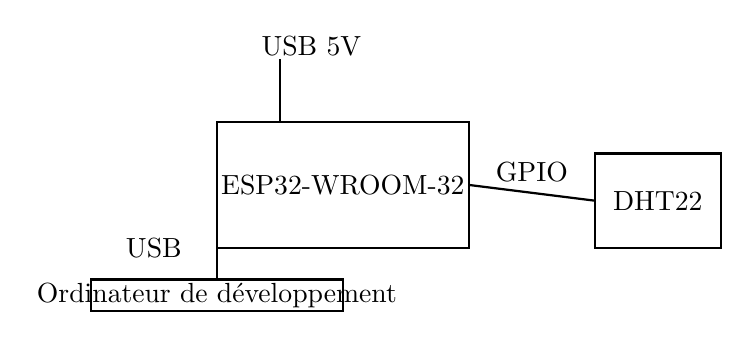
\begin{tikzpicture}[scale=0.8]
        % ESP32
        \draw[thick] (0,0) rectangle (4,2);
        \node at (2,1) {ESP32-WROOM-32};
        
        % DHT22
        \draw[thick] (6,0) rectangle (8,1.5);
        \node at (7,0.75) {DHT22};
        
        % Connexions
        \draw[thick] (4,1) -- (6,0.75);
        \node at (5,1.2) {GPIO};
        
        % Alimentation
        \draw[thick] (1,2) -- (1,3);
        \node at (1.5,3.2) {USB 5V};
        
        % PC
        \draw[thick] (-2,-1) rectangle (2,-0.5);
        \node at (0,-0.75) {Ordinateur de développement};
        
        % Connexion USB
        \draw[thick] (0,0) -- (0,-0.5);
        \node at (-1,0) {USB};
        
    \end{tikzpicture}
    \caption{Architecture matérielle Community Edition}
    \label{fig:hardware-architecture-community}
\end{figure}

\subsection{Diagramme de flux éducatif}

\begin{figure}[h]
    \centering
    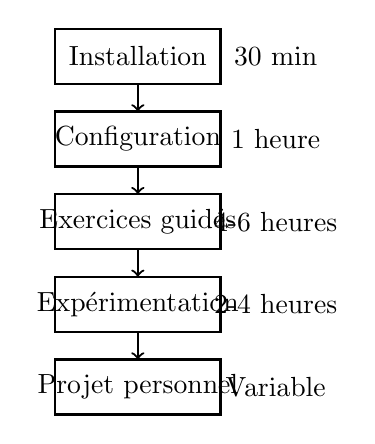
\begin{tikzpicture}[scale=0.7]
        % Boîtes
        \draw[thick] (0,6) rectangle (3,7) node[midway] {Installation};
        \draw[thick] (0,4.5) rectangle (3,5.5) node[midway] {Configuration};
        \draw[thick] (0,3) rectangle (3,4) node[midway] {Exercices guidés};
        \draw[thick] (0,1.5) rectangle (3,2.5) node[midway] {Expérimentation};
        \draw[thick] (0,0) rectangle (3,1) node[midway] {Projet personnel};
        
        % Flèches
        \draw[thick,->] (1.5,6) -- (1.5,5.5);
        \draw[thick,->] (1.5,4.5) -- (1.5,4);
        \draw[thick,->] (1.5,3) -- (1.5,2.5);
        \draw[thick,->] (1.5,1.5) -- (1.5,1);
        
        % Temps
        \node at (4,6.5) {30 min};
        \node at (4,5) {1 heure};
        \node at (4,3.5) {4-6 heures};
        \node at (4,2) {2-4 heures};
        \node at (4,0.5) {Variable};
        
    \end{tikzpicture}
    \caption{Flux d'apprentissage recommandé}
    \label{fig:learning-flow}
\end{figure}

\section{Résultats détaillés des tests}
\label{app:detailed-results}

\subsection{Métriques de performance complètes}

\begin{table}[h]
\centering
\caption{Résultats détaillés des tests de performance}
\label{tab:detailed-performance}
\begin{tabular}{|l|c|c|c|c|}
\hline
\textbf{Test} & \textbf{Min (ms)} & \textbf{Max (ms)} & \textbf{Moyenne (ms)} & \textbf{Écart-type} \\
\hline
SHA-256 (4KB) & 2.1 & 3.8 & 2.8 & 0.4 \\
ECDSA Sign & 45.2 & 67.3 & 52.1 & 5.8 \\
ECDSA Verify & 38.7 & 55.4 & 44.2 & 4.3 \\
Block Verification & 2.3 & 4.1 & 2.9 & 0.5 \\
Anomaly Detection & 12.4 & 18.7 & 15.1 & 2.1 \\
Random Generation (32B) & 0.9 & 1.6 & 1.2 & 0.2 \\
\hline
\end{tabular}
\end{table}

\subsection{Analyse statistique des faux positifs}

\begin{table}[h]
\centering
\caption{Distribution des faux positifs par cause}
\label{tab:false-positive-analysis}
\begin{tabular}{|l|c|c|c|}
\hline
\textbf{Cause} & \textbf{Occurrences} & \textbf{Pourcentage} & \textbf{Gravité} \\
\hline
Pics CPU temporaires & 15 & 34.9\% & Faible \\
Variations température & 10 & 23.3\% & Faible \\
Interférences Wi-Fi & 8 & 18.6\% & Moyenne \\
Fragmentation mémoire & 6 & 14.0\% & Faible \\
Autres causes & 4 & 9.3\% & Variable \\
\hline
\textbf{Total} & \textbf{43} & \textbf{100\%} & \\
\hline
\end{tabular}
\end{table}

\section{Guide d'installation détaillé}
\label{app:installation-guide}

\subsection{Prérequis système}

\textbf{Matériel requis :}
\begin{itemize}
    \item ESP32-WROOM-32 DevKit V1 (~5\$)
    \item DHT22 ou DHT11 (~3\$)
    \item Breadboard et câbles jumper (fourniture de base)
    \item Câble USB micro-B vers USB-A
    \item Ordinateur avec port USB libre
\end{itemize}

\textbf{Logiciels requis :}
\begin{itemize}
    \item ESP-IDF v4.4+ (gratuit)
    \item Python 3.7+ (généralement préinstallé)
    \item Pilotes USB-série (CP210x ou FTDI)
    \item Terminal série (intégré ESP-IDF)
\end{itemize}

\subsection{Procédure d'installation étape par étape}

\textbf{Étape 1 : Installation ESP-IDF}
\begin{enumerate}
    \item Télécharger ESP-IDF depuis le site officiel Espressif
    \item Suivre le guide d'installation pour votre OS
    \item Vérifier l'installation avec \texttt{idf.py --version}
\end{enumerate}

\textbf{Étape 2 : Configuration matérielle}
\begin{enumerate}
    \item Connecter DHT22 : VCC → 3.3V, GND → GND, Data → GPIO4
    \item Vérifier les connexions avec un multimètre si disponible
    \item Connecter ESP32 au PC via USB
\end{enumerate}

\textbf{Étape 3 : Compilation et flash}
\begin{enumerate}
    \item Cloner le repository SecureIoT-VIF Community
    \item \texttt{cd secureiot-vif-community}
    \item \texttt{idf.py build}
    \item \texttt{idf.py -p /dev/ttyUSB0 flash monitor}
\end{enumerate}

\section{Exercices pratiques}
\label{app:exercises}

\subsection{Exercice 1 : Configuration de base}

\textbf{Objectif :} Installer et configurer SecureIoT-VIF Community Edition

\textbf{Prérequis :} Installation ESP-IDF complète

\textbf{Durée estimée :} 45 minutes

\textbf{Instructions :}
\begin{enumerate}
    \item Suivre le guide d'installation (Annexe \ref{app:installation-guide})
    \item Compiler et flasher le firmware de base
    \item Observer les logs de démarrage sécurisé
    \item Identifier les messages de vérification d'intégrité
    \item Documenter les temps de démarrage mesurés
\end{enumerate}

\textbf{Questions de réflexion :}
\begin{itemize}
    \item Quelles sont les étapes de la chaîne de confiance observées ?
    \item Quel est l'impact du framework sur le temps de démarrage ?
    \item Comment les clés cryptographiques sont-elles générées ?
\end{itemize}

\subsection{Exercice 2 : Manipulation des seuils}

\textbf{Objectif :} Comprendre la détection d'anomalies par seuils fixes

\textbf{Prérequis :} Exercice 1 complété avec succès

\textbf{Durée estimée :} 90 minutes

\textbf{Instructions :}
\begin{enumerate}
    \item Modifier les seuils dans \texttt{secureiot\_config.h}
    \item Recompiler et reflasher
    \item Simuler des conditions anormales :
    \begin{itemize}
        \item Chauffer l'ESP32 (sèche-cheveux) pour trigger le seuil température
        \item Lancer des boucles intensives pour surcharger le CPU
        \item Allouer de la mémoire pour trigger le seuil mémoire
    \end{itemize}
    \item Observer et analyser les alertes générées
    \item Tester différentes valeurs de seuils
\end{enumerate}

\textbf{Questions de réflexion :}
\begin{itemize}
    \item Comment choisir des seuils appropriés ?
    \item Quels sont les avantages et inconvénients des seuils fixes ?
    \item Comment réduire les faux positifs ?
\end{itemize}

\subsection{Exercice 3 : Simulation d'attaques}

\textbf{Objectif :} Comprendre la détection de modifications de firmware

\textbf{Prérequis :} Exercices 1 et 2 complétés

\textbf{Durée estimée :} 2 heures

\textbf{Instructions :}
\begin{enumerate}
    \item Calculer le hash initial du firmware avec l'outil fourni
    \item Modifier artificiellement quelques bytes dans la flash
    \item Observer la détection lors de la vérification périodique
    \item Analyser les logs de détection d'intégrité
    \item Restaurer le firmware original
    \item Répéter avec différents types de modifications
\end{enumerate}

\textbf{Attaques à simuler :}
\begin{itemize}
    \item Modification d'un seul byte
    \item Modification de plusieurs bytes consécutifs
    \item Modification dans différentes sections (code, données, config)
    \item Injection de code simple (NOP slides)
\end{itemize}

\section{Ressources complémentaires}
\label{app:resources}

\subsection{Liens utiles}

\textbf{Documentation officielle :}
\begin{itemize}
    \item ESP-IDF Programming Guide : \url{https://docs.espressif.com/projects/esp-idf/}
    \item mbedTLS Documentation : \url{https://tls.mbed.org/}
    \item FreeRTOS Reference : \url{https://freertos.org/Documentation/}
\end{itemize}

\textbf{Communautés et forums :}
\begin{itemize}
    \item ESP32 Community Forum : \url{https://esp32.com/}
    \item Reddit r/esp32 : \url{https://reddit.com/r/esp32}
    \item Stack Overflow ESP32 Tag : \url{https://stackoverflow.com/questions/tagged/esp32}
\end{itemize}

\subsection{Bibliographie spécialisée}

Pour approfondir les concepts abordés dans SecureIoT-VIF Community Edition, nous recommandons la lecture des ouvrages et articles suivants :

\textbf{Sécurité IoT générale :}
\begin{itemize}
    \item "IoT Penetration Testing Cookbook" par Aaron Guzman
    \item "Practical IoT Hacking" par Fotios Chantzis
    \item "Building Secure Firmware" par Kai Michaelis
\end{itemize}

\textbf{Cryptographie embarquée :}
\begin{itemize}
    \item "A Graduate Course in Applied Cryptography" par Dan Boneh
    \item "Embedded Security in Cars" par Lemke, Paar, Wolf
    \item Publications récentes sur la cryptographie légère et post-quantique
\end{itemize}

\section{Licence et contribution}
\label{app:license}

\subsection{Licence d'utilisation}

SecureIoT-VIF Community Edition est distribué sous licence MIT, permettant :
\begin{itemize}
    \item Utilisation libre à des fins éducatives et de recherche
    \item Modification et redistribution avec attribution
    \item Utilisation commerciale avec les restrictions appropriées
    \item Contribution communautaire encouragée
\end{itemize}

\subsection{Comment contribuer}

Les contributions au projet SecureIoT-VIF Community Edition sont les bienvenues :

\textbf{Types de contributions appréciées :}
\begin{itemize}
    \item Corrections de bugs et améliorations du code
    \item Nouveaux exercices pédagogiques et scénarios
    \item Traductions de la documentation
    \item Portage vers d'autres plateformes (Arduino, Raspberry Pi)
    \item Amélioration de la documentation utilisateur
\end{itemize}

\textbf{Processus de contribution :}
\begin{enumerate}
    \item Fork du repository principal
    \item Création d'une branche dédiée pour la fonctionnalité
    \item Développement avec tests appropriés
    \item Documentation des modifications
    \item Pull request avec description détaillée
\end{enumerate}

Cette approche collaborative assure l'évolution continue du framework pour bénéficier à toute la communauté éducative en sécurité IoT.